\documentclass[12pt, twoside]{article}
\usepackage[letterpaper, margin=1in, headsep=0.5in]{geometry}
\usepackage[english]{babel}
\usepackage[utf8]{inputenc}
\usepackage{amsmath}
\usepackage{amsfonts}
\usepackage{amssymb}
\usepackage{tikz}
\usetikzlibrary{quotes, angles}
\usepackage{graphicx}
\usepackage{multicol}

%\usepackage{pgfplots}
%\pgfplotsset{width=10cm,compat=1.9}
%\usepgfplotslibrary{statistics}
%\usepackage{pgfplotstable}
%\usepackage{tkz-fct}
%\usepackage{venndiagram}

\usepackage{fancyhdr}
\pagestyle{fancy}
\fancyhf{}
\renewcommand{\headrulewidth}{0pt} % disable the underline of the header

\fancyhead[RE]{\thepage}
\fancyhead[RO]{\thepage \\ Name: \hspace{3cm}}
\fancyhead[L]{BECA / Dr. Huson / Geometry 10th Grade\\* Unit 1: Introduction to Geometry\\13 September 2019}

\begin{document}
\subsubsection*{1.7 Exam: Spicy problems for early finishers}
  \vspace{0.25cm}
  \begin{enumerate}

  \item Given $\overline{ABC}$, $AB=4$, and $AC=25$.\\ [0.5cm]
  Find ${BC}$.\\[1.5cm]
      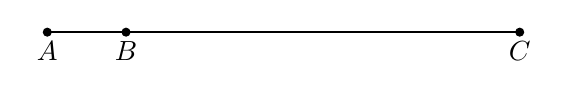
\begin{tikzpicture}
        \draw [-, thick] (1,0)--(7,0);
        \draw [fill] (1,0) circle [radius=0.05] node[below]{$A$};
        \draw [fill] (2,0) circle [radius=0.05] node[below]{$B$};
        \draw [fill] (7,0) circle [radius=0.05] node[below]{$C$};
      \end{tikzpicture} \vspace{2cm}

    \item Given $\overleftrightarrow{PQ}$ as shown on the number line, with $P=-3$ and $Q=5.5$. \\[20pt] % Midpoint
    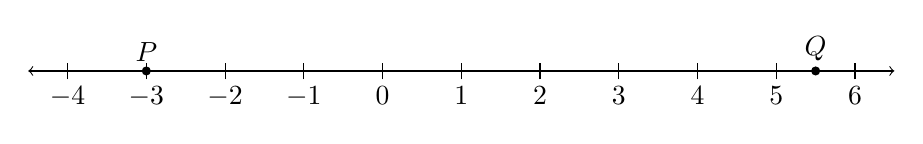
\begin{tikzpicture}
      \draw [<->] (-4.5,0)--(6.5,0);
      \foreach \x in {-4,...,6} %2 leading for diff!=1
        \draw[shift={(\x,0)},color=black] (0pt,-3pt) -- (0pt,3pt) node[below=5pt]  {$\x$};
        \draw [fill] (-3,0) circle [radius=0.05] node[above] {$P$};
        \draw [fill] (5.5,0) circle [radius=0.05] node[above] {$Q$};
    \end{tikzpicture} \\ \bigskip
    What is the exact distance on the number line between the points $P$ and $Q$? \vspace{2cm}  

    \item Given the rectangle $ABCD$ shown below, with $AB=12$ and $BC=5$. The diagonal $\overline{AC}$ is drawn to create two triangles. Find the area of the lower triangle, $\triangle ABC$.
    \begin{flushleft}
    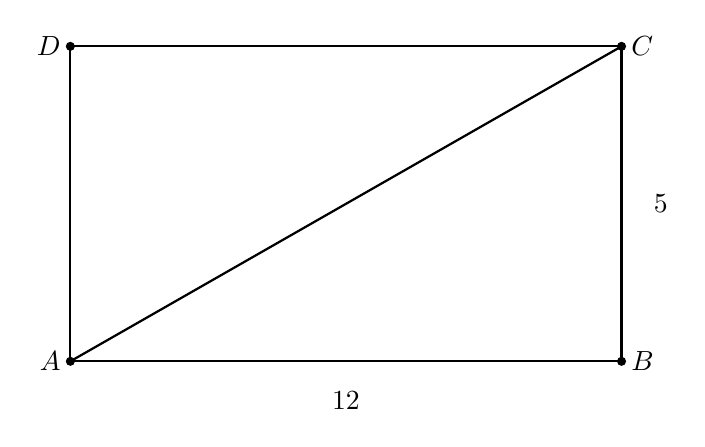
\begin{tikzpicture}
      \draw [-, thick] (0,0)--(7,0)--(7,4)--(0,4)--cycle;
      \draw [-, thick] (0,0)--(7,4);
      \draw [fill] (0,0) circle [radius=0.05] node[left]{$A$};
      \draw [fill] (7,0) circle [radius=0.05] node[right]{$B$};
      \draw [fill] (7,4) circle [radius=0.05] node[right]{$C$};
      \draw [fill] (0,4) circle [radius=0.05] node[left]{$D$};
      \node at (7.5, 2){5};
      \node at (3.5, -0.5){12};
    \end{tikzpicture}
    \end{flushleft}

    \newpage

    \item Given $\overline{WXYZ}$, $WX=3 \frac{1}{2}$, $XY=4 \frac{3}{4}$, and $YZ= 1 \frac{1}{4}$. \\ [0.25cm]
    Find ${WZ}$.\\[.5in]
        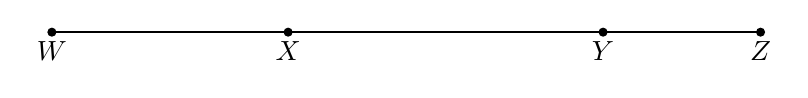
\begin{tikzpicture}
          \draw [-, thick] (0,0)--(9,0);
          \draw [fill] (0,0) circle [radius=0.05] node[below]{$W$};
          \draw [fill] (3,0) circle [radius=0.05] node[below]{$X$};
          \draw [fill] (7,0) circle [radius=0.05] node[below]{$Y$};
          \draw [fill] (9,0) circle [radius=0.05] node[below]{$Z$};
        \end{tikzpicture} \vspace{1cm}
      
    \item A student constructs a triangle with a given side, $\overline{AB}$ as shown below. Is $\triangle ABC$ equilateral? Justify your answer by explaining what was done incorrectly and how it should have been done.
    \begin{flushleft}
    \begin{tikzpicture}[scale=0.7, rotate=-20]
      \draw [-, thick] (0,0)--(5,0)--(66.4:4)--cycle;
      \draw [fill] (0,0) circle [radius=0.05] node[left]{$A$};
      \draw [fill] (5,0) circle [radius=0.05] node[right]{$B$};
      \draw [fill] (66.4:4) circle [radius=0.05] node[above]{$C$};
      \draw (0,0) circle [radius=4];
      \draw (5,0) circle [radius=5];
    \end{tikzpicture}
    \end{flushleft}
    \vspace{1cm}

    \item In the following two problems, solve for the value of $x$ by factoring.
  \begin{multicols}{2}
    \begin{enumerate}
      \item   $x^2+6x=-5$ \vspace{6cm}
      \item   $x^2=x+12$ \vspace{6cm}
    \end{enumerate}
  \end{multicols}
    \vspace{3cm}


  \end{enumerate}
\end{document}
